% - integrate SIR model (use UML diagrams)
% - visualization
% - impoistance computation
% - run tests

After having used the Vadere software with its existing features, we have to implement a new feature by adding the SIR (Susceptible-Infectious-Removed) model into the source code \cite{vadere-source}. Firstly, we need to set up our development environment. We used IntelliJ IDEA as our IDE and the latest Java development kit (OpenJDK). We copied the SIR files provided to us on Moodle and pasted them at the proper locations as specified by the first line of each file. In order to run it, we first have to rebuild the software and also do a clean maven build.
\textbf{Figure \ref{fig:UMLDiagram}} shows the UML diagram representing all the new classes that have been included for the SIR model. We go into more details for each file now:
\begin{figure}
  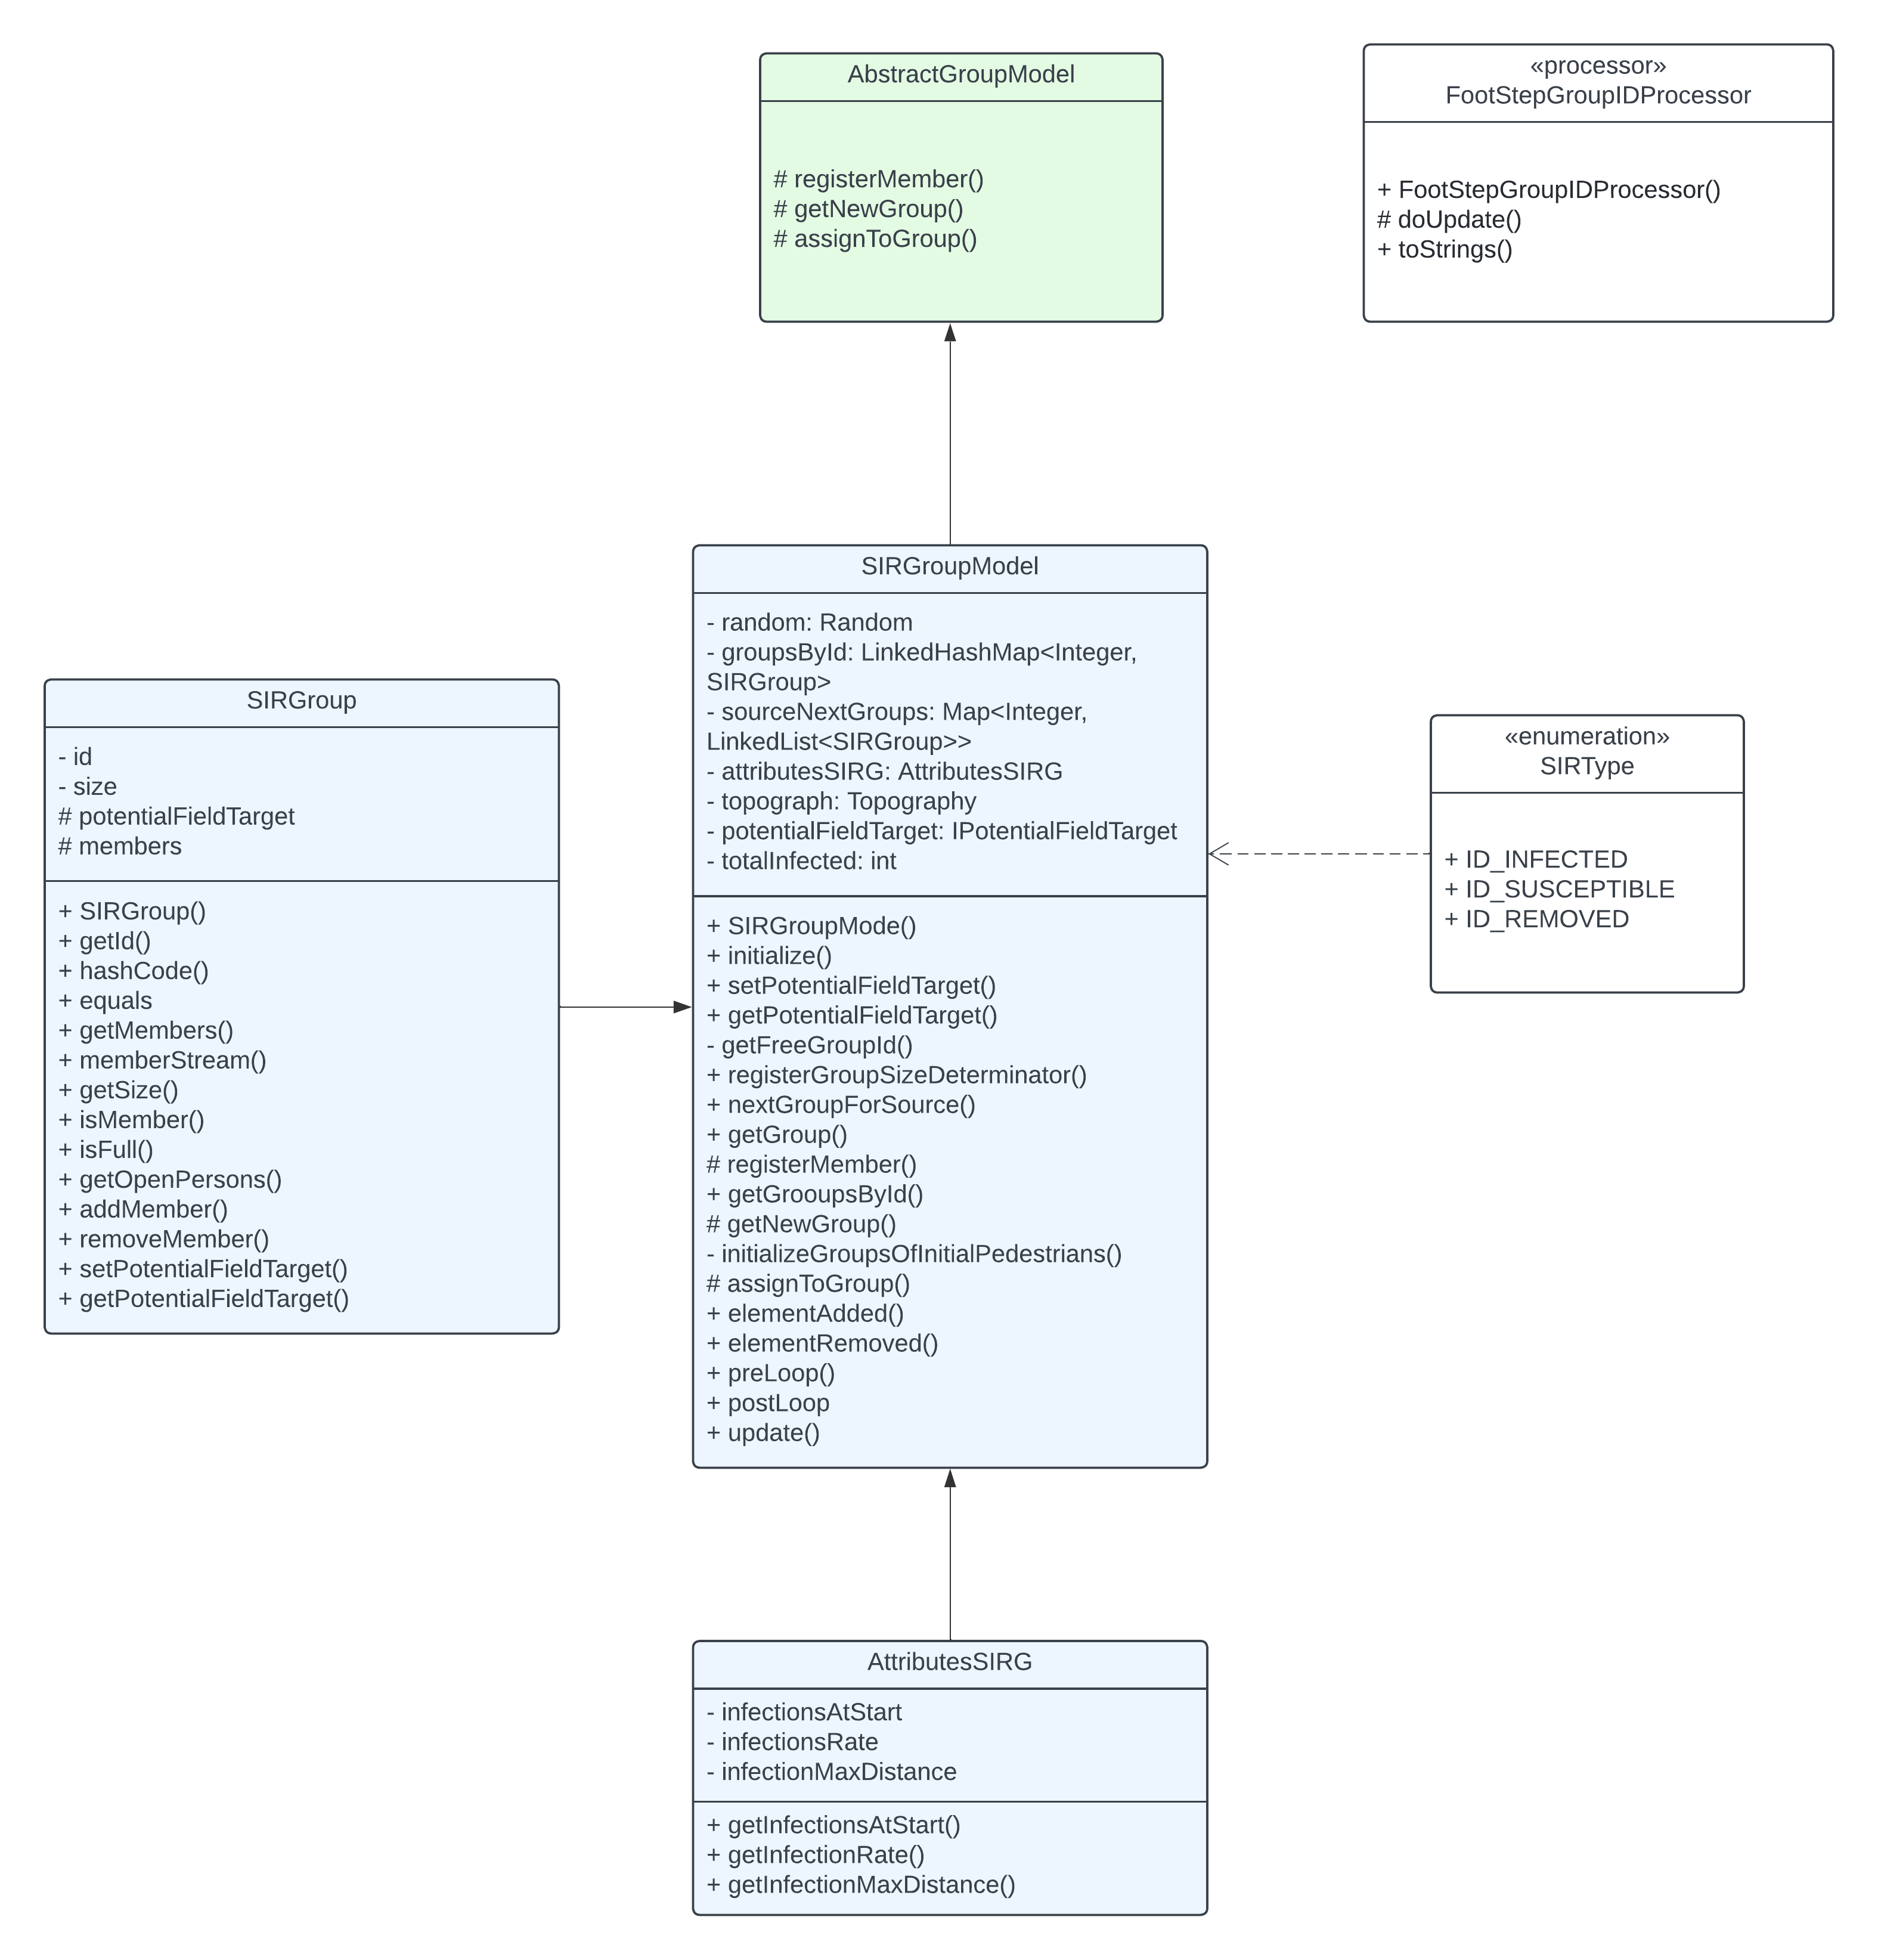
\includegraphics[width=\linewidth]{images/UML class.png}
  \caption{UML diagram representing SIR class}
  \label{fig:UMLDiagram}
\end{figure}
\begin{itemize}
\item \textbf{AbstractGroupModel}: An abstract that serves as the base for implementing various group models in the Vadere software. \\
\textbf{\texttt{{Methods:}}}
\begin{itemize}
    \item \textit{registerMember(Pedestrian ped, T currentGroup):} An abstract method for registering a pedestrian to a specified group.
    \item \textit{getNewGroup(int size):} An abstract method for obtaining a new group with the given size.
    \item \textit{getNewGroup(final int id, final int size):} An abstract method for obtaining a new group with the specified ID and size.
    \item \textit{assignToGroup(Pedestrian pedestrian):} An abstract method for assigning a pedestrian to a group.
\end{itemize}

\item \textbf{AttributesSIRG}: This class extends the \texttt{Attributes class} and is used to define the attributes specific to the SIR model. \\
\textbf{\texttt{{Methods:}}}
\begin{itemize}
    \item \textit{getInfectionsAtStart():} Returns the value of \texttt{infectionsAtStart} attribute.
    \item \textit{getInfectionRate():} Returns the value of \texttt{infectionRate} attribute.
    \item \textit{getInfectionMaxDistance():}Returns the value of \texttt{infectionMaxDistance} attribute.
\end{itemize}

\item \textbf{FootStepGroupIDProcessor}: This class extends \texttt{DataProcessor<EventtimePedestrianIdKey, Integer>} and implements the \texttt{ModelFilter} interface. This class is a data processor designed to extract and process information related to group IDs based on footstep data. \\
\textbf{\texttt{{Methods:}}}
\begin{itemize}
    \item \textit{doUpdate(SimulationState state):} It updates the processor based on the simulation state. For each group, it iterates over group members and footstep data to extract and associate group IDs with pedestrianIds and event times.
    \item \textit{toStrings(EventtimePedestrianIdKey key):} It converts the data associated with a given key into a string array.
\end{itemize}

\item \textbf{SIRType}: This file defines enumeration for different types of individuals within the context of the SIR model which consists of \texttt{ID\_INFECTED}, \texttt{ID\_SUSCEPTIBLE} and \texttt{ID\_REMOVED}.
\item \textbf{SIRGroup}:This file represents a SIR Group. \\
\textbf{\texttt{{Methods:}}}
\begin{itemize}
    \item \textit{getId():} Returns group ID.
    \item \textit{equals(Group o):} Compares with another group based on their IDs.
    \item \textit{getMembers():} Returns a list of pedestrians who are members of the group.
    \item \textit{getSize():}Returns the size of the group
    \item \textit{isMember(Pedestrian ped):} Checks if a pedestrian is a member of the group.
    \item \textit{isFull():} Checks if the group is full.
    \item \textit{getOpenPersons():} Returns the number of remaining spots in the group.
    \item \textit{addMember() and removeMember():} Adds or remove a pedestrian
    \item \textit{setPotentialFieldTarget():} Sets the potetntial field target for the group.
    \item \textit{getPotentialFieldTarget():} Returns the potetntial field target for the group.
\end{itemize}
\item \textbf{SIRGroupModel}:This file implements the SIR Group model. \\
\textbf{\texttt{{Methods:}}}
\begin{itemize}
    \item \textit{initialize():} Initializes the SIR group model with required attributes.
    \item \textit{setPotentialFieldTarget() and getPotentialFieldTarget():} Sets or returns the potential field target for the group model.
    \item \textit{getFreeGroupId():} Determines a free group ID based on infectionRate and total infected pedestrians.
    \item \textit{getGroup():} Reutrns the SIR group of the pedestrian. 
    \item \textit{isMember(Pedestrian ped):} Checks if a pedestrian is a member of the group.
    \item \textit{registerMember():} Registers a pedestrian as a member of a specific SIR group.
    \item \textit{getNewGroup():} Overloaded function to return either a free group ID or create a new one.
    \item \textit{assignToGroup():} Overloaded function to assign a pedestrian to a specific SIR group or a free SIR group.
    \item \textit{elementAdded() and elementRemoved():} Adds or remove a pedestrian from a group.
    \item \textit{update():} Updates the SIR groups and simulate infections.
    
\end{itemize}
\end{itemize}

\textit{\textbf{Correct colour visualization:}} Currently, the colours are not visualised correctly for different groups (infected, susceptible, removed). In order to do that, we modified the class \texttt{SimulationModel.java} to include different colours for different groups. Figure \ref{fig:SIRGroupColoring} shows the highlighted code that has been changed to include the colours for different groups. We chose red for infected, blue for susceptible, and green for removed. This change only allows us to see the groups during the simulation and does not work for post-visualization.
\begin{figure}[H]
    \centering
    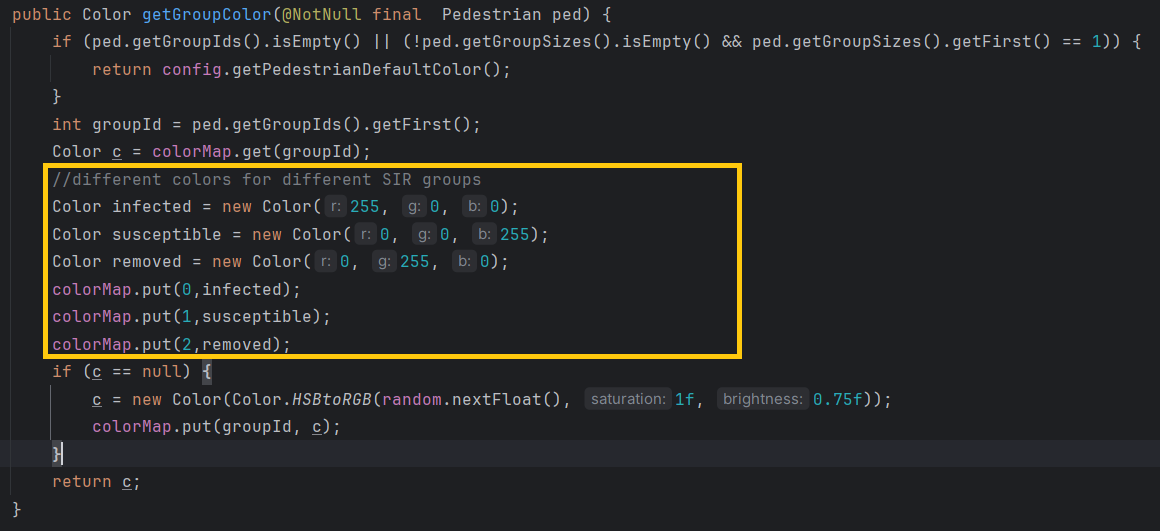
\includegraphics[width=\linewidth]{images/SIRGroupColoring.png}
    \caption{Modified code for different groups}
    \label{fig:SIRGroupColoring}
\end{figure}





\textit{\textbf{Increasing Efficiency in  Distance Computation:}}

If we look into the \texttt{LinkedCellsGrid.java} file we can see that \texttt{getObjects} is used to retrieve pedestrians near to an infected pedestrian. This function basically looks at every cell of the \texttt{grid}. If there is any object in that cell, it will then compare distances to the center. In the end, this function adds pedestrians who are nearer or equal to the radius to the \texttt{result} variable, which will be used later with the \texttt{infectionRate} attribute to decide whether selected pedestrians are infected or not.

While this method gives correct results, it does not necessarily mean that it cannot be advanced and made more efficient. If the number of pedestrians increases for each group, it can be observed that the number of computations increases. For $n$ number of pedestrians, if we look at the whole grid for them, we would get $O(n*width*height)$ as time complexity, which will be computationally intensive.

When we searched for a better solution, we found out that the \texttt{Quadtree} data structure is the best way to implement this function as it is on a map. 

Basically, as explained by \href{https://www.youtube.com/watch?v=OELWhbqaUWQ}{AJT}, \texttt{Quadtree} uses both Binary Trees and Recursion to achieve its purpose. While, only leaf nodes store relevant data, root nodes and internal nodes store information to get these data. Internal nodes contain 4 pointers to point to directions of the current point: Northeast, Northwest, Southeast, and Southwest. When someone wants to reach a location, they need to go through quadrant nodes until they get to the leaf node. 

So compared to looking at the whole grid, it is more efficient to go through nodes and find the point that we want to reach. It has a time complexity of $O(log(n))$ for searching, which proves that compared to the previous method, it is much more efficient.

However, this method also has flaws. In some situations, if points are near to each other they may cause too much recursion of nodes, as can be seen in figure \ref{fig:subfig6}. However, it can be still said that in most of the situations with spread pedestrians, \texttt{Quadtree} data structure helped us to improve the efficiency.

\begin{figure}
\begin{center}
    \centering
    \begin{subfigure}{\textwidth}
        \centering
        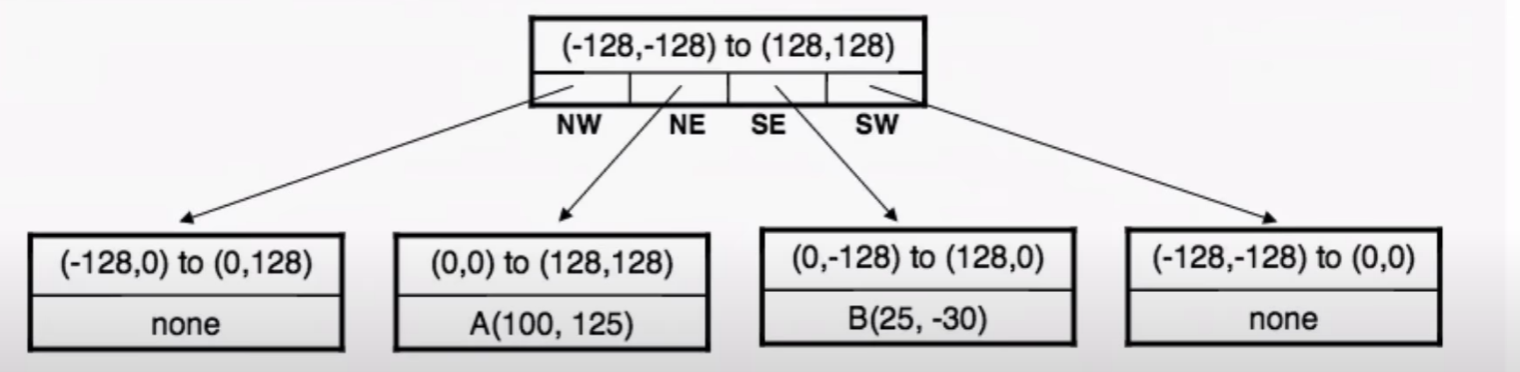
\includegraphics[width=\linewidth]{images/task4_quad1.png}
        \label{fig:subfig1}
    \end{subfigure}
    \caption{How \texttt{QuadTree} works. Pointer for 4 sections. Internal nodes do not store information for data}
\end{center}
\end{figure}


\begin{center}
\begin{figure}[H]
    \centering
    \begin{subfigure}[t]{0.38\textwidth}
        \centering
        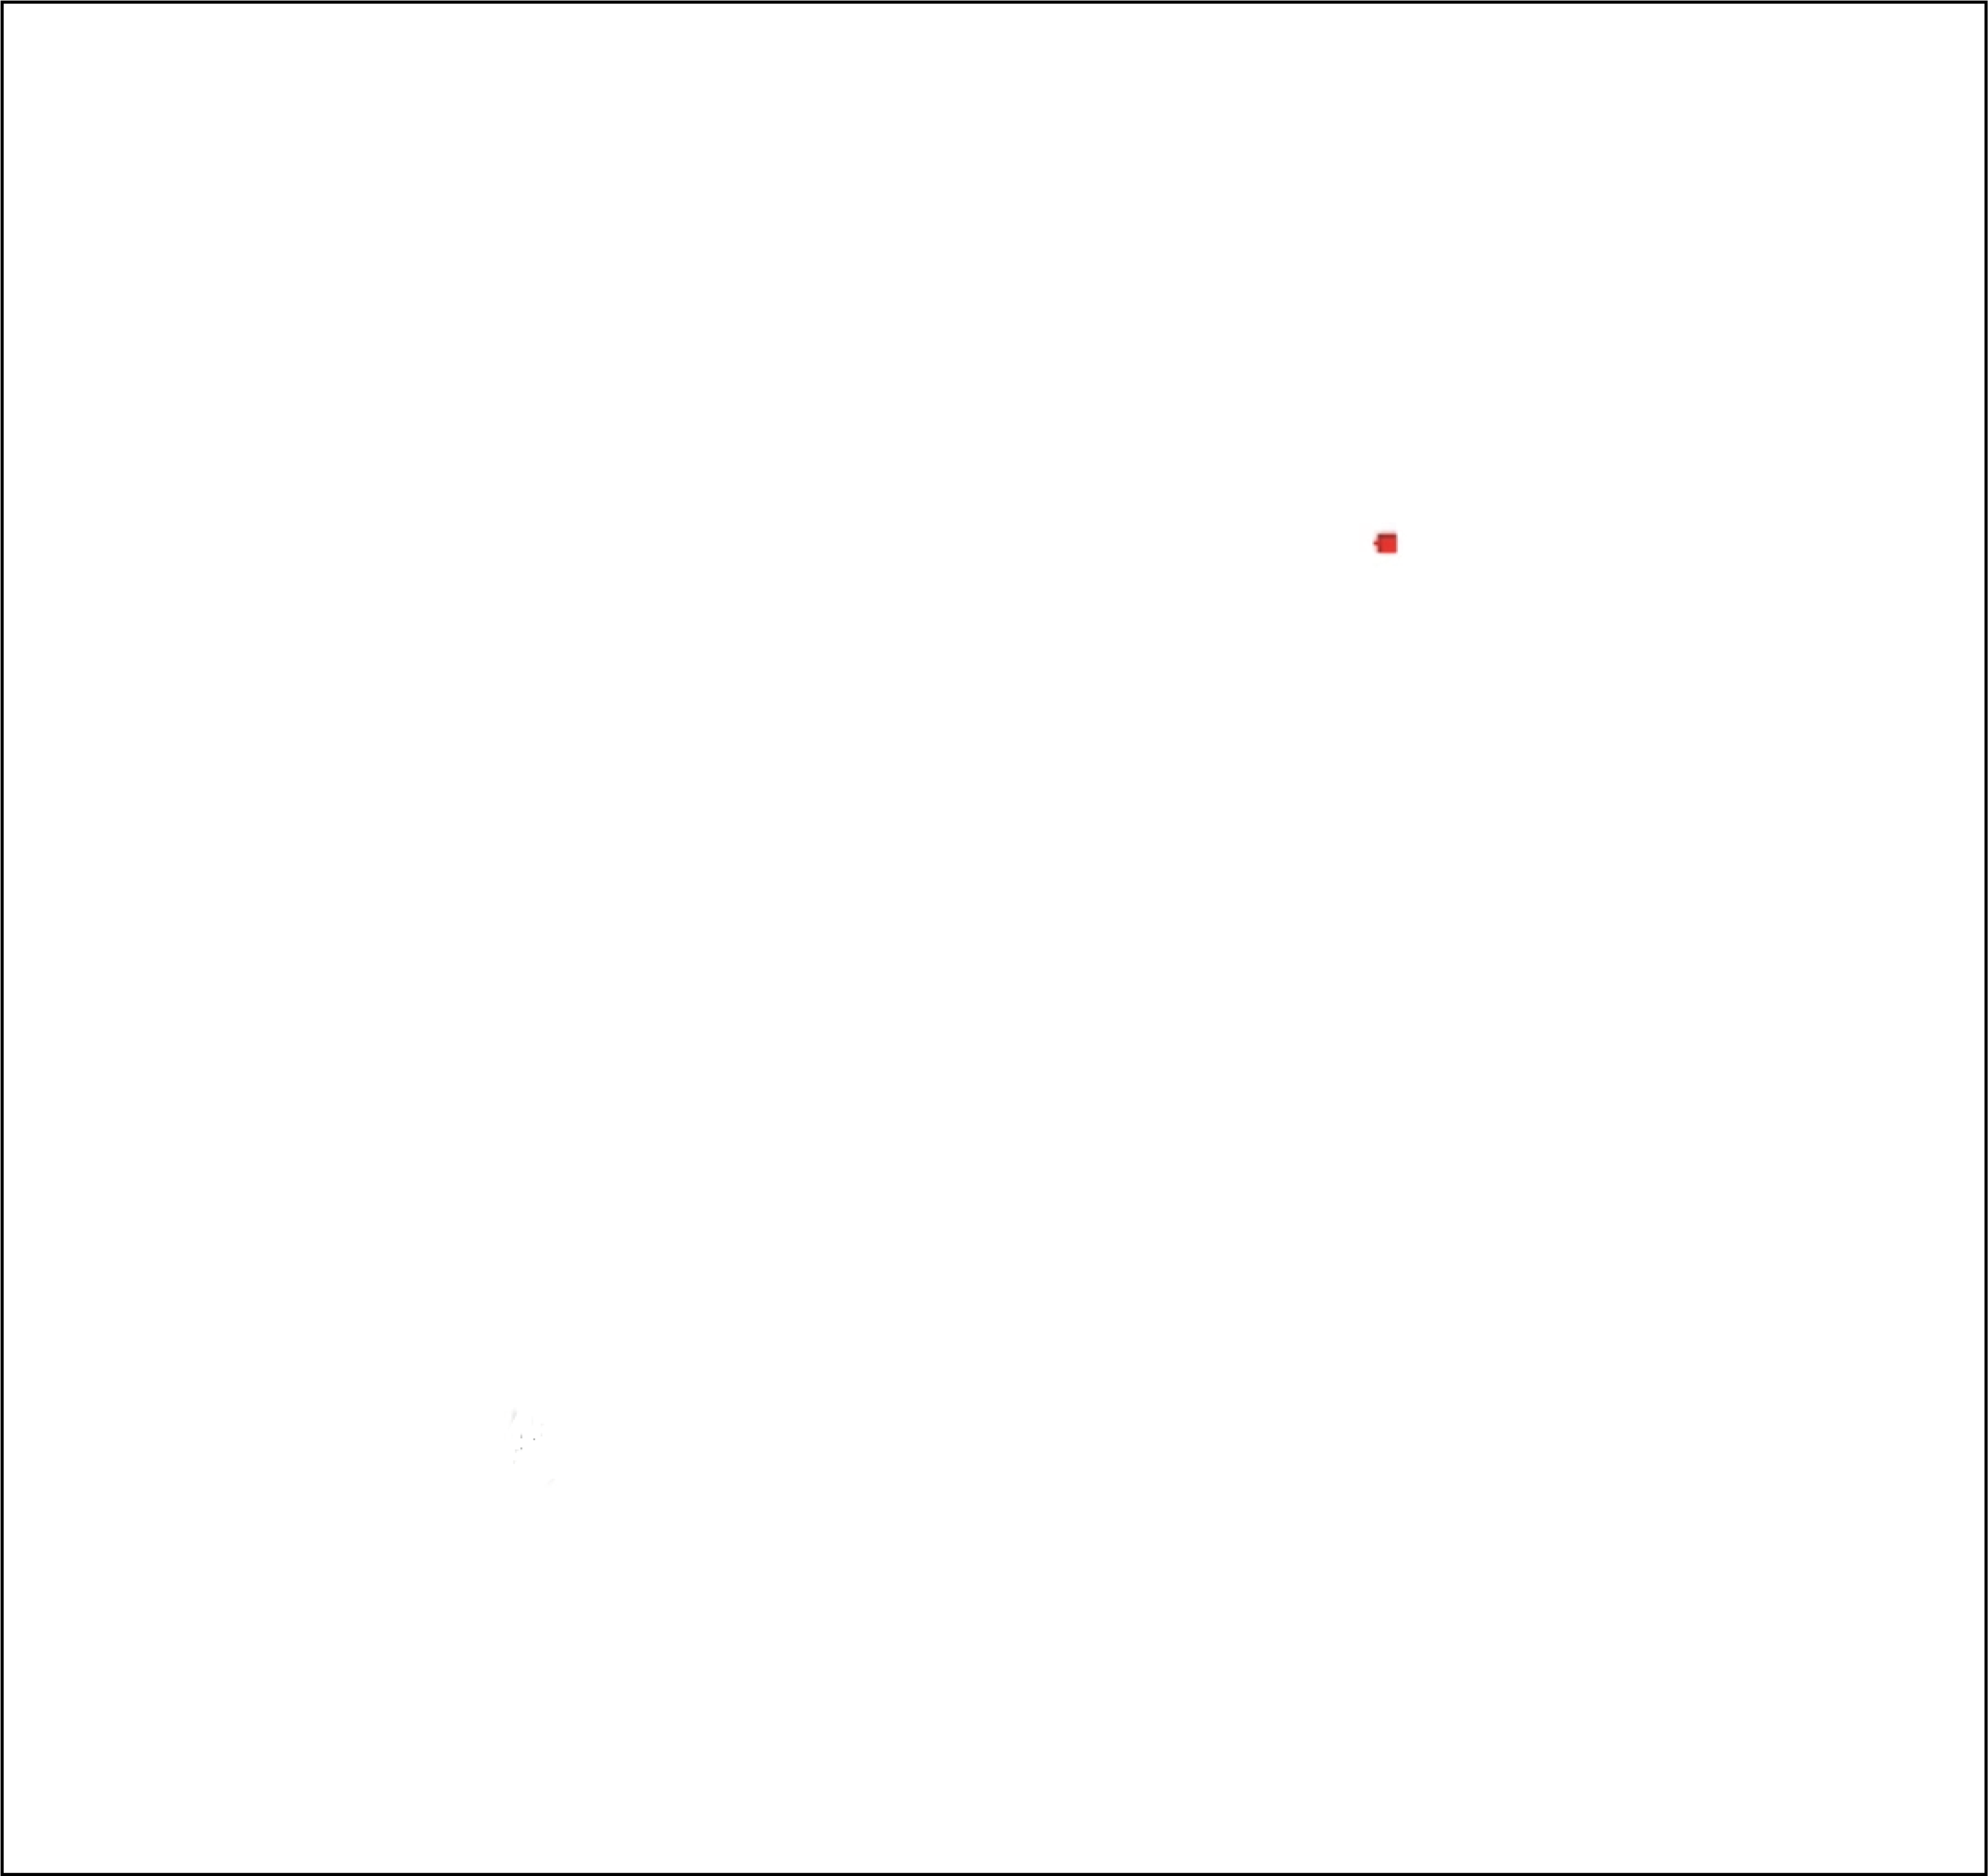
\includegraphics[width=\linewidth]{images/task4_quad2.png}
        \caption{If there is only one point, there is no need to separate the area into places. One node is enough.}
        \label{fig:subfig2}
    \end{subfigure}%
    \hspace{0.02\textwidth}
    \begin{subfigure}[t]{0.38\textwidth}
        \centering
        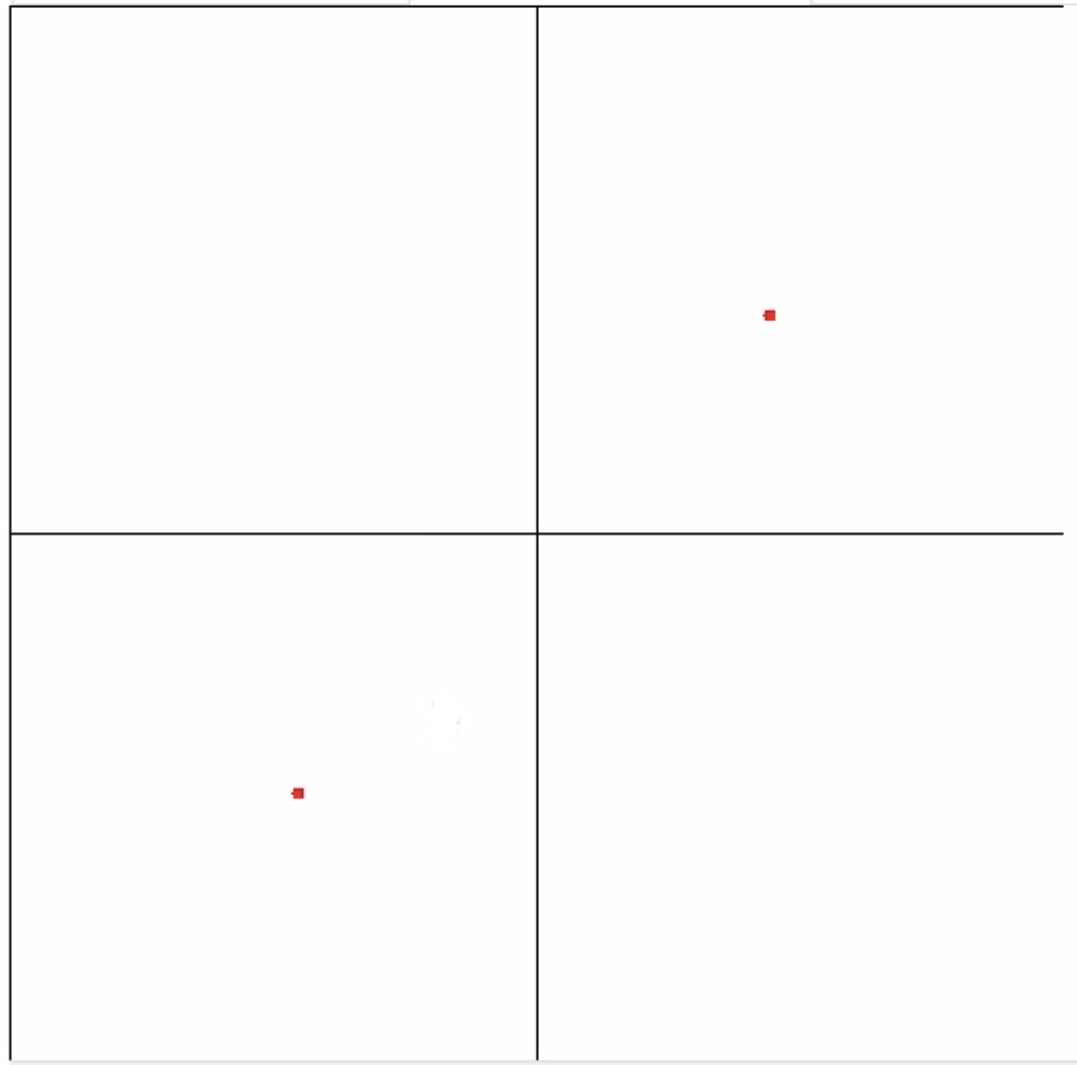
\includegraphics[width=\linewidth]{images/task4_quad3.png}
        \caption{If we put another point to another place, \texttt{QuadTree} will divide the total area into 4 pieces. The root node will have a pointer to these two points. The other 2 leaf nodes will be empty.}
        \label{fig:subfig3}
    \end{subfigure}

    \centering
    \begin{subfigure}[t]{0.38\textwidth}
        \centering
        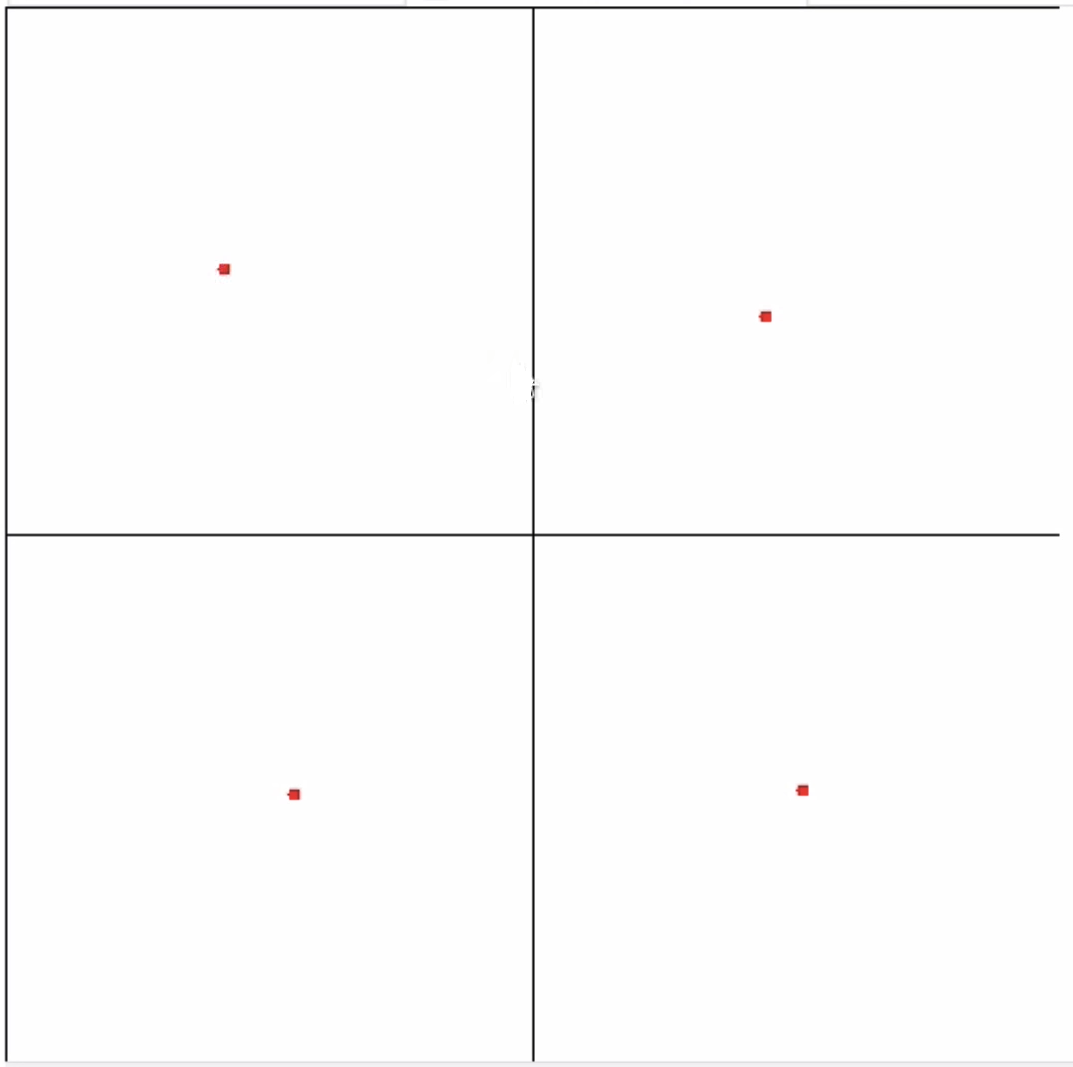
\includegraphics[width=\linewidth]{images/task4_quad4.png}
        \caption{ If we keep putting a point into an empty node, it will not scale the tree again}
        \label{fig:subfig4}
    \end{subfigure}%
    \hspace{0.02\textwidth}
    \begin{subfigure}[t]{0.38\textwidth}
        \centering
        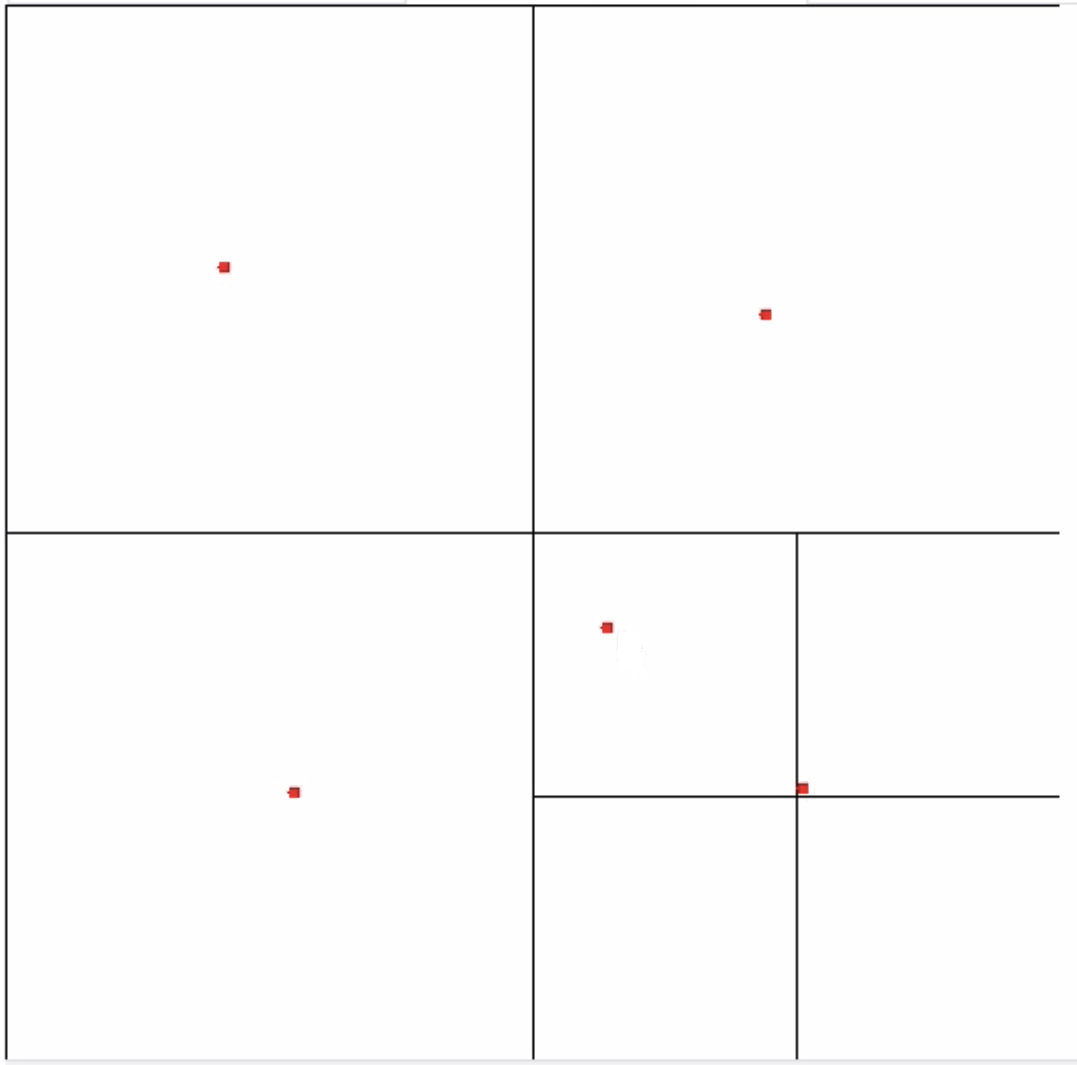
\includegraphics[width=\linewidth]{images/task4_quad5.png}
        \caption{When we put the fifth point properly, the root node will have a pointer to another internal node which contains a pointer to 4 leaf nodes. }
        \label{fig:subfig5}
    \end{subfigure}

    \caption{\texttt{QuadTree} Visualization}
\end{figure}


\begin{figure}[H]\ContinuedFloat
    \centering
    \begin{subfigure}{0.38\textwidth}
        \centering
        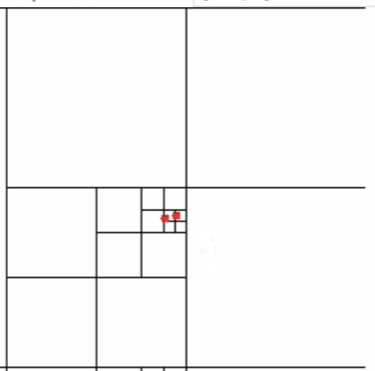
\includegraphics[width=\linewidth]{images/task4_quad6.png}
        \caption{Flaw of \texttt{QuadTree}. If we put two points too close to each other, it may cause unnecessary creation of internal nodes while only 2 of them have pointers to data available leaf nodes. }
        \label{fig:subfig6}
    \end{subfigure}
    \caption{\texttt{QuadTree} Visualization}
\end{figure}
\end{center}











\textit{\textbf{Decoupling simulation step size from infection rate:}} In the current implementation, the infection rate depends on the simulation step size. However, this is not desirable as a change in simulation step size also changes the infection behaviour. For this reason, it is desirable to decouple them. Although it is very hard to perfectly decouple them because simulation always depends on some degree of time discretisation, we try to decouple them as far as possible. Figure \ref{fig:decoupling} includes the highlighted lines of code that we have added to try and achieve this aim. We added a new attribute \texttt{elapsedTime} to check and allow for simulation to happen only when \texttt{1} second has passed from the previous simulation. This reduces the effect of \texttt{simulation time step} and makes the simulation behaviour more realistic.
\begin{figure}[H]
    \centering
    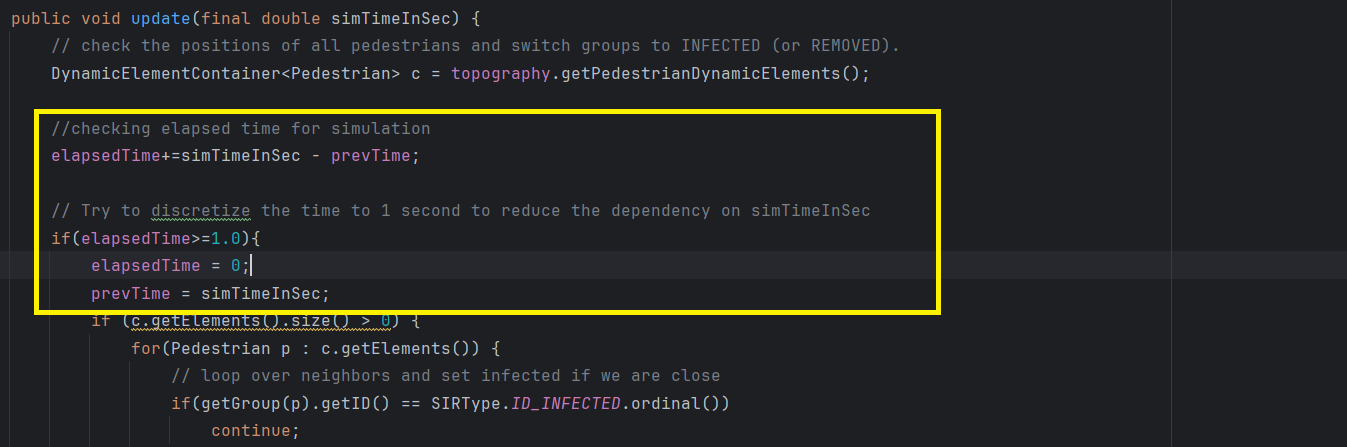
\includegraphics[width = \linewidth]{images/decoupling.png}
    \caption{Decoupling simulation time step from infection rate}
    \label{fig:decoupling}
\end{figure}

\textit{\textbf{Static experiments:}} After making all the changes to the code, we ran some experiments with our modified code as mentioned in the exercise sheet:
\begin{itemize}
    \item \textbf{Scenario 1}: A static scenario with 1000 pedestrians randomly distributed in the scenario. For this scenario, we started with the following attributes:
    \begin{itemize}
        \item \texttt{infectionsAtStart}: 0
        \item \texttt{infectionRate}: 0.05
        \item \texttt{infectionsMaxDistance}: 1.0
    \end{itemize}
    Figure \ref{fig:task4.5_1} shows the simulation progress from start to end with pedestrians slowly getting infected over time until all the pedestrians are infected at the end. We used the \textit{Dash/Plotly visulalization} tool to visualize the simulation results. Figure \ref{fig:task4.5_1_visualization} shows the graph of pedestrians getting infected where half of the pedestrians got infected in around \texttt{19} seconds.
    \item \textbf{Scenario 2}: Now we have to double the \texttt{infectionRate} from that of the previous experiment. So we set the \texttt{infectionRate} to \texttt{0.1} while keeping the other attributes the same and run the experiment again. 
    This time, for half of the pedestrians to get infected it took around \texttt{7} seconds which is less than half of the time it took in the first setting.
    Figure \ref{fig:task4.5_2_visualization} shows the graph with both settings. We can easily see that it took way less time for pedestrians to get infected when the \texttt{infectionRate} was increased.
\end{itemize}

\begin{figure}[H]
    \centering
   \begin{subfigure}{0.3\textwidth}
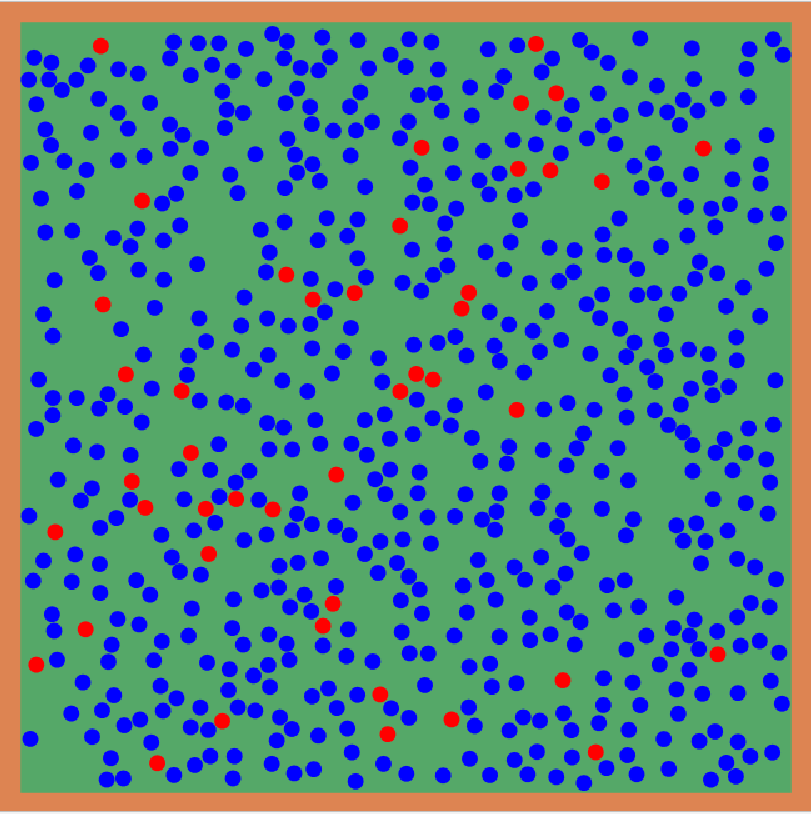
\includegraphics[width=\textwidth]{images/task4.5_start.png}
    \label{fig:start}
    \caption{start}
\end{subfigure}
   \begin{subfigure}{0.3\textwidth}
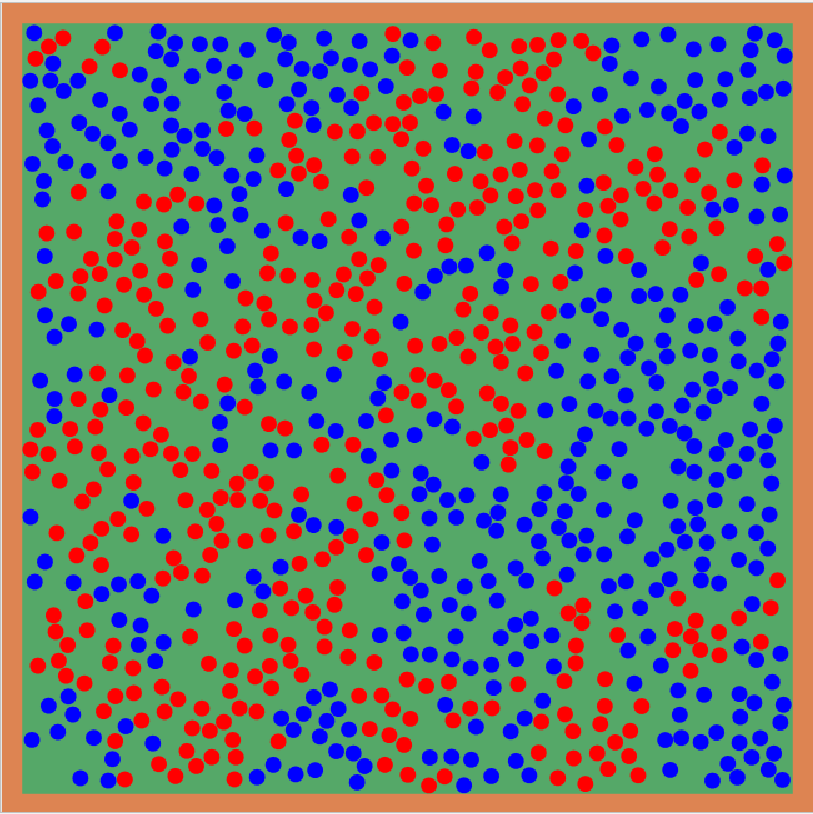
\includegraphics[width=\textwidth]{images/task4.5_mid.png}
    \label{fig:mid}
    \caption{middle}
\end{subfigure}
   \begin{subfigure}{0.3\textwidth}
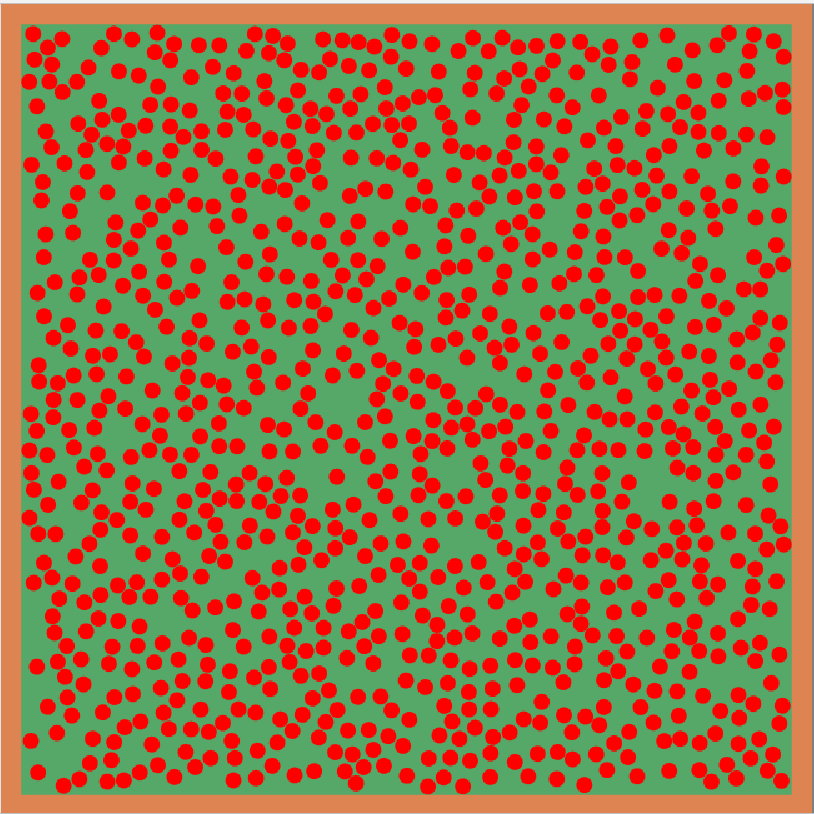
\includegraphics[width=\textwidth]{images/task4.5_end.png}
    \label{fig:end}
    \caption{End}
\end{subfigure}
    \caption{Simulation Progress}
    \label{fig:task4.5_1}
\end{figure}

\begin{figure}[H]
    \centering
   \begin{subfigure}{\textwidth}
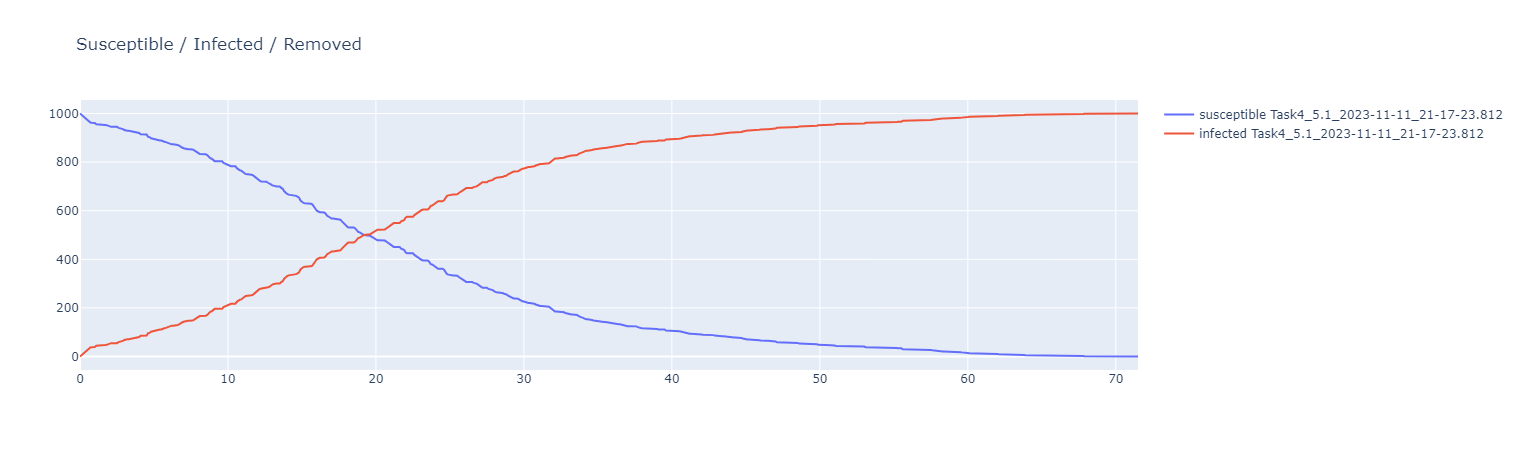
\includegraphics[width=\textwidth]{images/task4.5_1_simulation.png}
 \caption{Infection Rate: 0.05}
    \label{fig:task4.5_1_visualization}
\end{subfigure}
\end{figure}

\begin{figure}[H]\ContinuedFloat



   \begin{subfigure}{\textwidth}
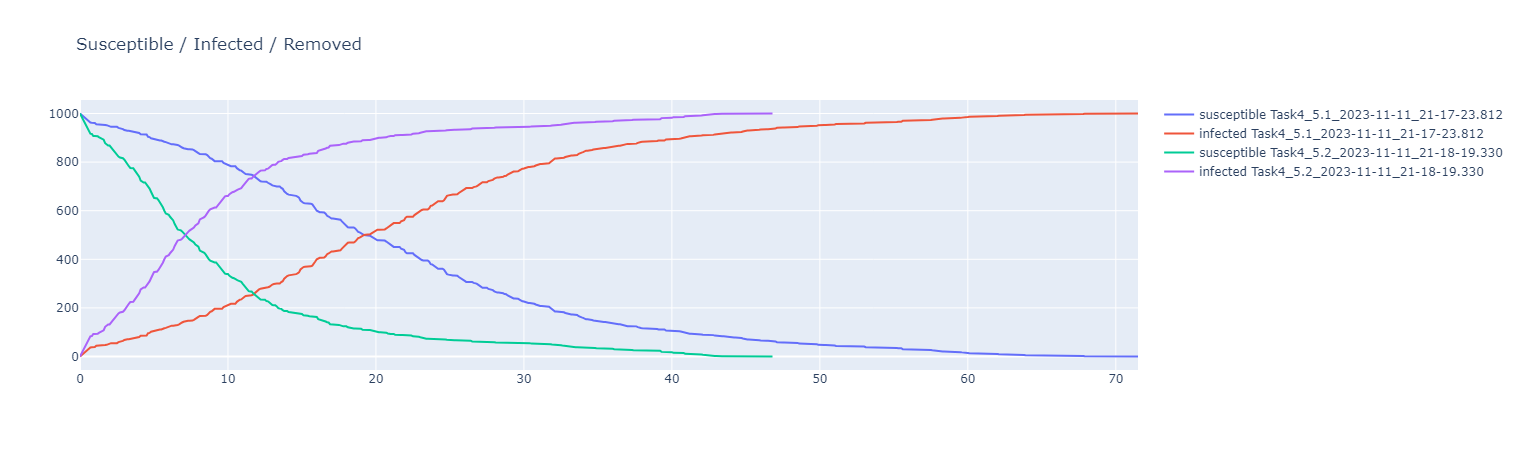
\includegraphics[width=\textwidth]{images/task4.5_2_simulation.png}
 \caption{Comparison between infection rates 0.05 and 0.1}
    \label{fig:task4.5_2_visualization}
\end{subfigure}
    \caption{Visualization of different infection rates}
    \label{fig:task4.5_Visualization}
\end{figure}

% \\
% \\
% \\

 \textit{\textbf{Corridor Scenario:}} We implement a 40m x 20m corridor scenario where 100 pedestrians move from right to left and another 100 move from left to right. With an infection rate of 0.1, it can be seen from Figure \ref{fig:task4_graph_cor} that not all pedestrians get infected. Out of 200 people, only \textbf{137} of them are infected, and the acceleration of infection decreases significantly after the contact of the different directioned groups ends. If we increase the number of pedestrians, length of the corridor, or \texttt{infectionRate}, it can be observed that the number of infections will increase.
 
\begin{figure}[H]
    \centering
    
    \begin{subfigure}{0.4\textwidth}
        \centering
        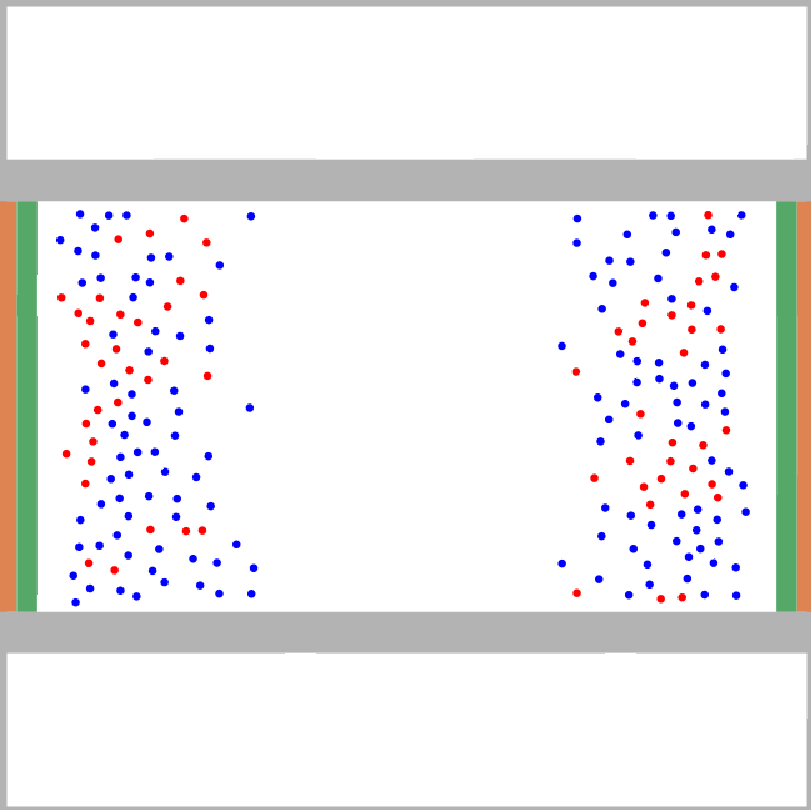
\includegraphics[width=\textwidth]{images/task4_cooridor.png}
        \caption{Pedestrians in different directions approach each other. Some of them are infected}
    \end{subfigure}
      \hspace{0.05\textwidth}
    \begin{subfigure}{0.4\textwidth}
        \centering
        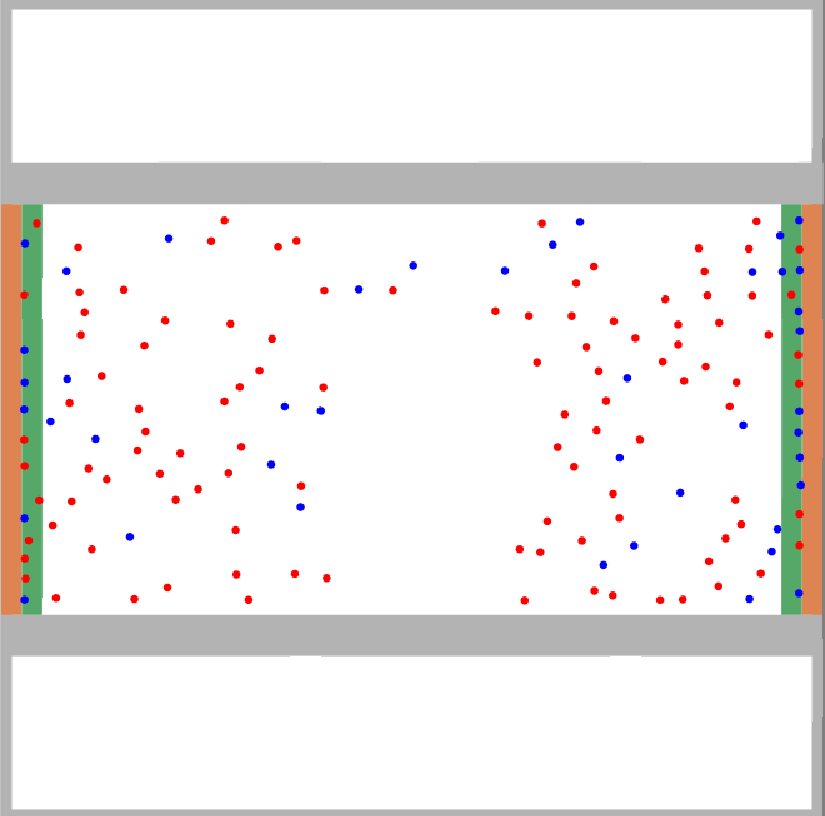
\includegraphics[width=\textwidth]{images/task4_cooridor2.png}
        \caption{Distribution of susceptible and infected pedestrians after collision ends }
    \end{subfigure}
    
    \begin{subfigure}{\textwidth}
        \centering
        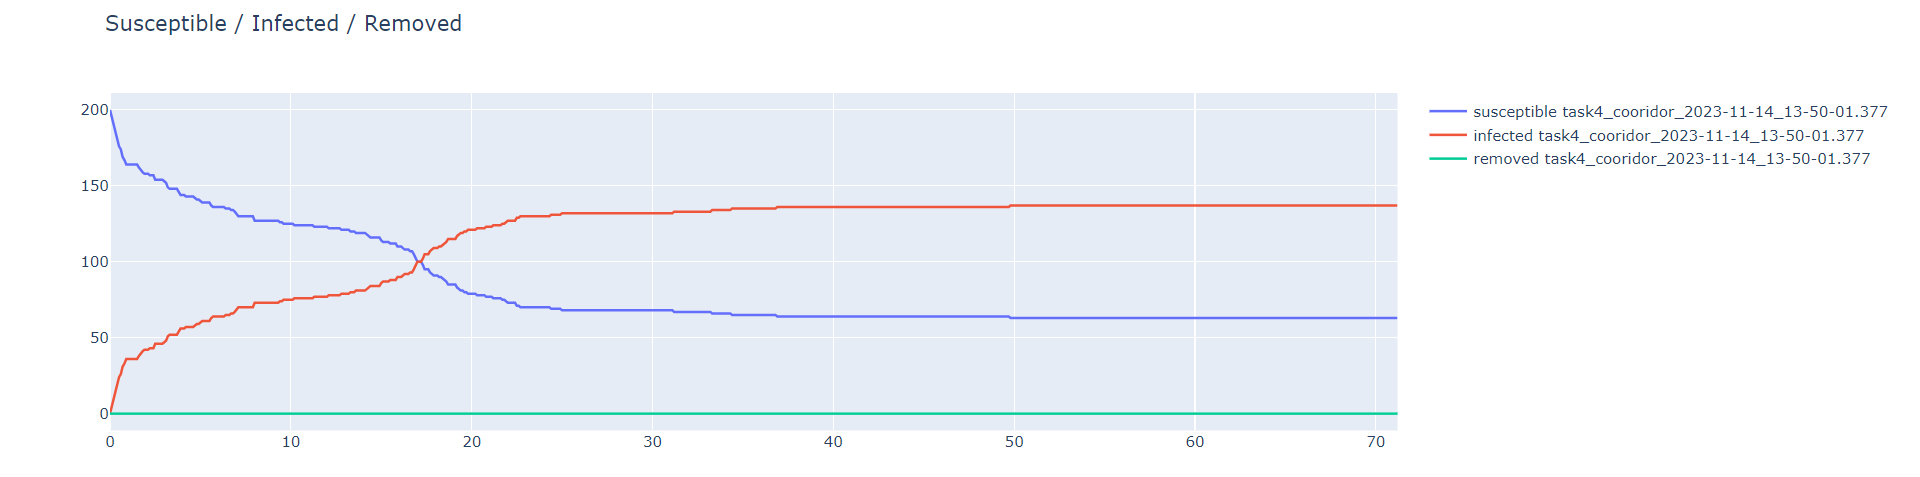
\includegraphics[width=\linewidth]{images/task4_cooridor1.png}
        \caption{Pedestrian Groups (Infected \& Susceptible) / Time Graph. At the beginning and at the contact time between different directioned pedestrians, acceleration of infection is high compared to other points.}
        \label{fig:task4_graph_cor}
    \end{subfigure}
    
    \caption{Corridor Scenario of 40m × 20m}
\end{figure}





 \textit{\textbf{Possible Extensions:}} \\
In order to make our model more realistic, here are some suggested extensions that can be added:\newline
\begin{itemize}
    \item \textit{\textbf{Age Groups: }}Every demography has people of different age groups with different immunity strengths. For example, younger people tend to have better immunity and faster recovery rates than older people and hence they are less susceptible to getting infected. Adding the age parameter to \texttt{Pedestrian} and giving different \texttt{infectionRate} and \texttt{recoveryRate} would make our model more robust and realistic. 
    \item \textit{\textbf{Adding vaccinated groups: }}Another nice extension to our SIR model would be to add a certain percentage of the population to be \texttt{vaccinated} by adding this attribute to the \texttt{Pedestrian}. The vaccinated groups would be significantly less susceptible to getting infected or having a faster or greater chance of recovery in case they are infected.
    \item \textit{\textbf{Incubation period for exposed individuals:} }Adding another group of \texttt{exposed} individuals can also be beneficial regarding realism. Exposed individuals who have been infected do not start to show the symptoms right away and have lower chances of infecting others. Adding the \texttt{exposed} group with an \texttt{incubationPeriod} time which is the time after which they actually get sick and start showing symptoms can make our model more realistic. 
\end{itemize}

 